\begin{table}[htbp]\centering\small
\caption{Known-truth binary simulation of the unchanged sign-aware/MoM rule. Each row uses 500 repetitions, $n=2000$ and two-fold AIPW with logistic working models. The non-null ATE is computed by quadrature.}\label{tab:simulation-results}
\begin{tabularx}{\textwidth}{Xrrrrr}\toprule Scenario & True ATE & Raw RMSE & Signed RMSE & Coverage & Reject 0 \\\midrule
Matched controls & 0.000 & 0.123 & 0.028 & 0.952 & 0.048 \\
Matched controls & 0.105 & 0.124 & 0.027 & 0.954 & 0.960 \\
Different magnitudes & 0.000 & 0.123 & 0.082 & 0.228 & 0.772 \\
Different magnitudes & 0.105 & 0.124 & 0.081 & 0.230 & 0.184 \\
Incompatible factors & 0.000 & 0.147 & 0.347 & 0.000 & 1.000 \\
Incompatible factors & 0.111 & 0.146 & 0.345 & 0.000 & 1.000 \\
No confounding & 0.000 & 0.024 & 0.025 & 0.948 & 0.052 \\
No confounding & 0.105 & 0.023 & 0.024 & 0.960 & 0.988 \\
\bottomrule\end{tabularx}\end{table}
At coverage 0.95, Monte Carlo standard error is about 0.010 for 500 repetitions. Rejection at true zero measures type-I error; at nonzero effects it measures power. 
\begin{figure}[htbp]\centering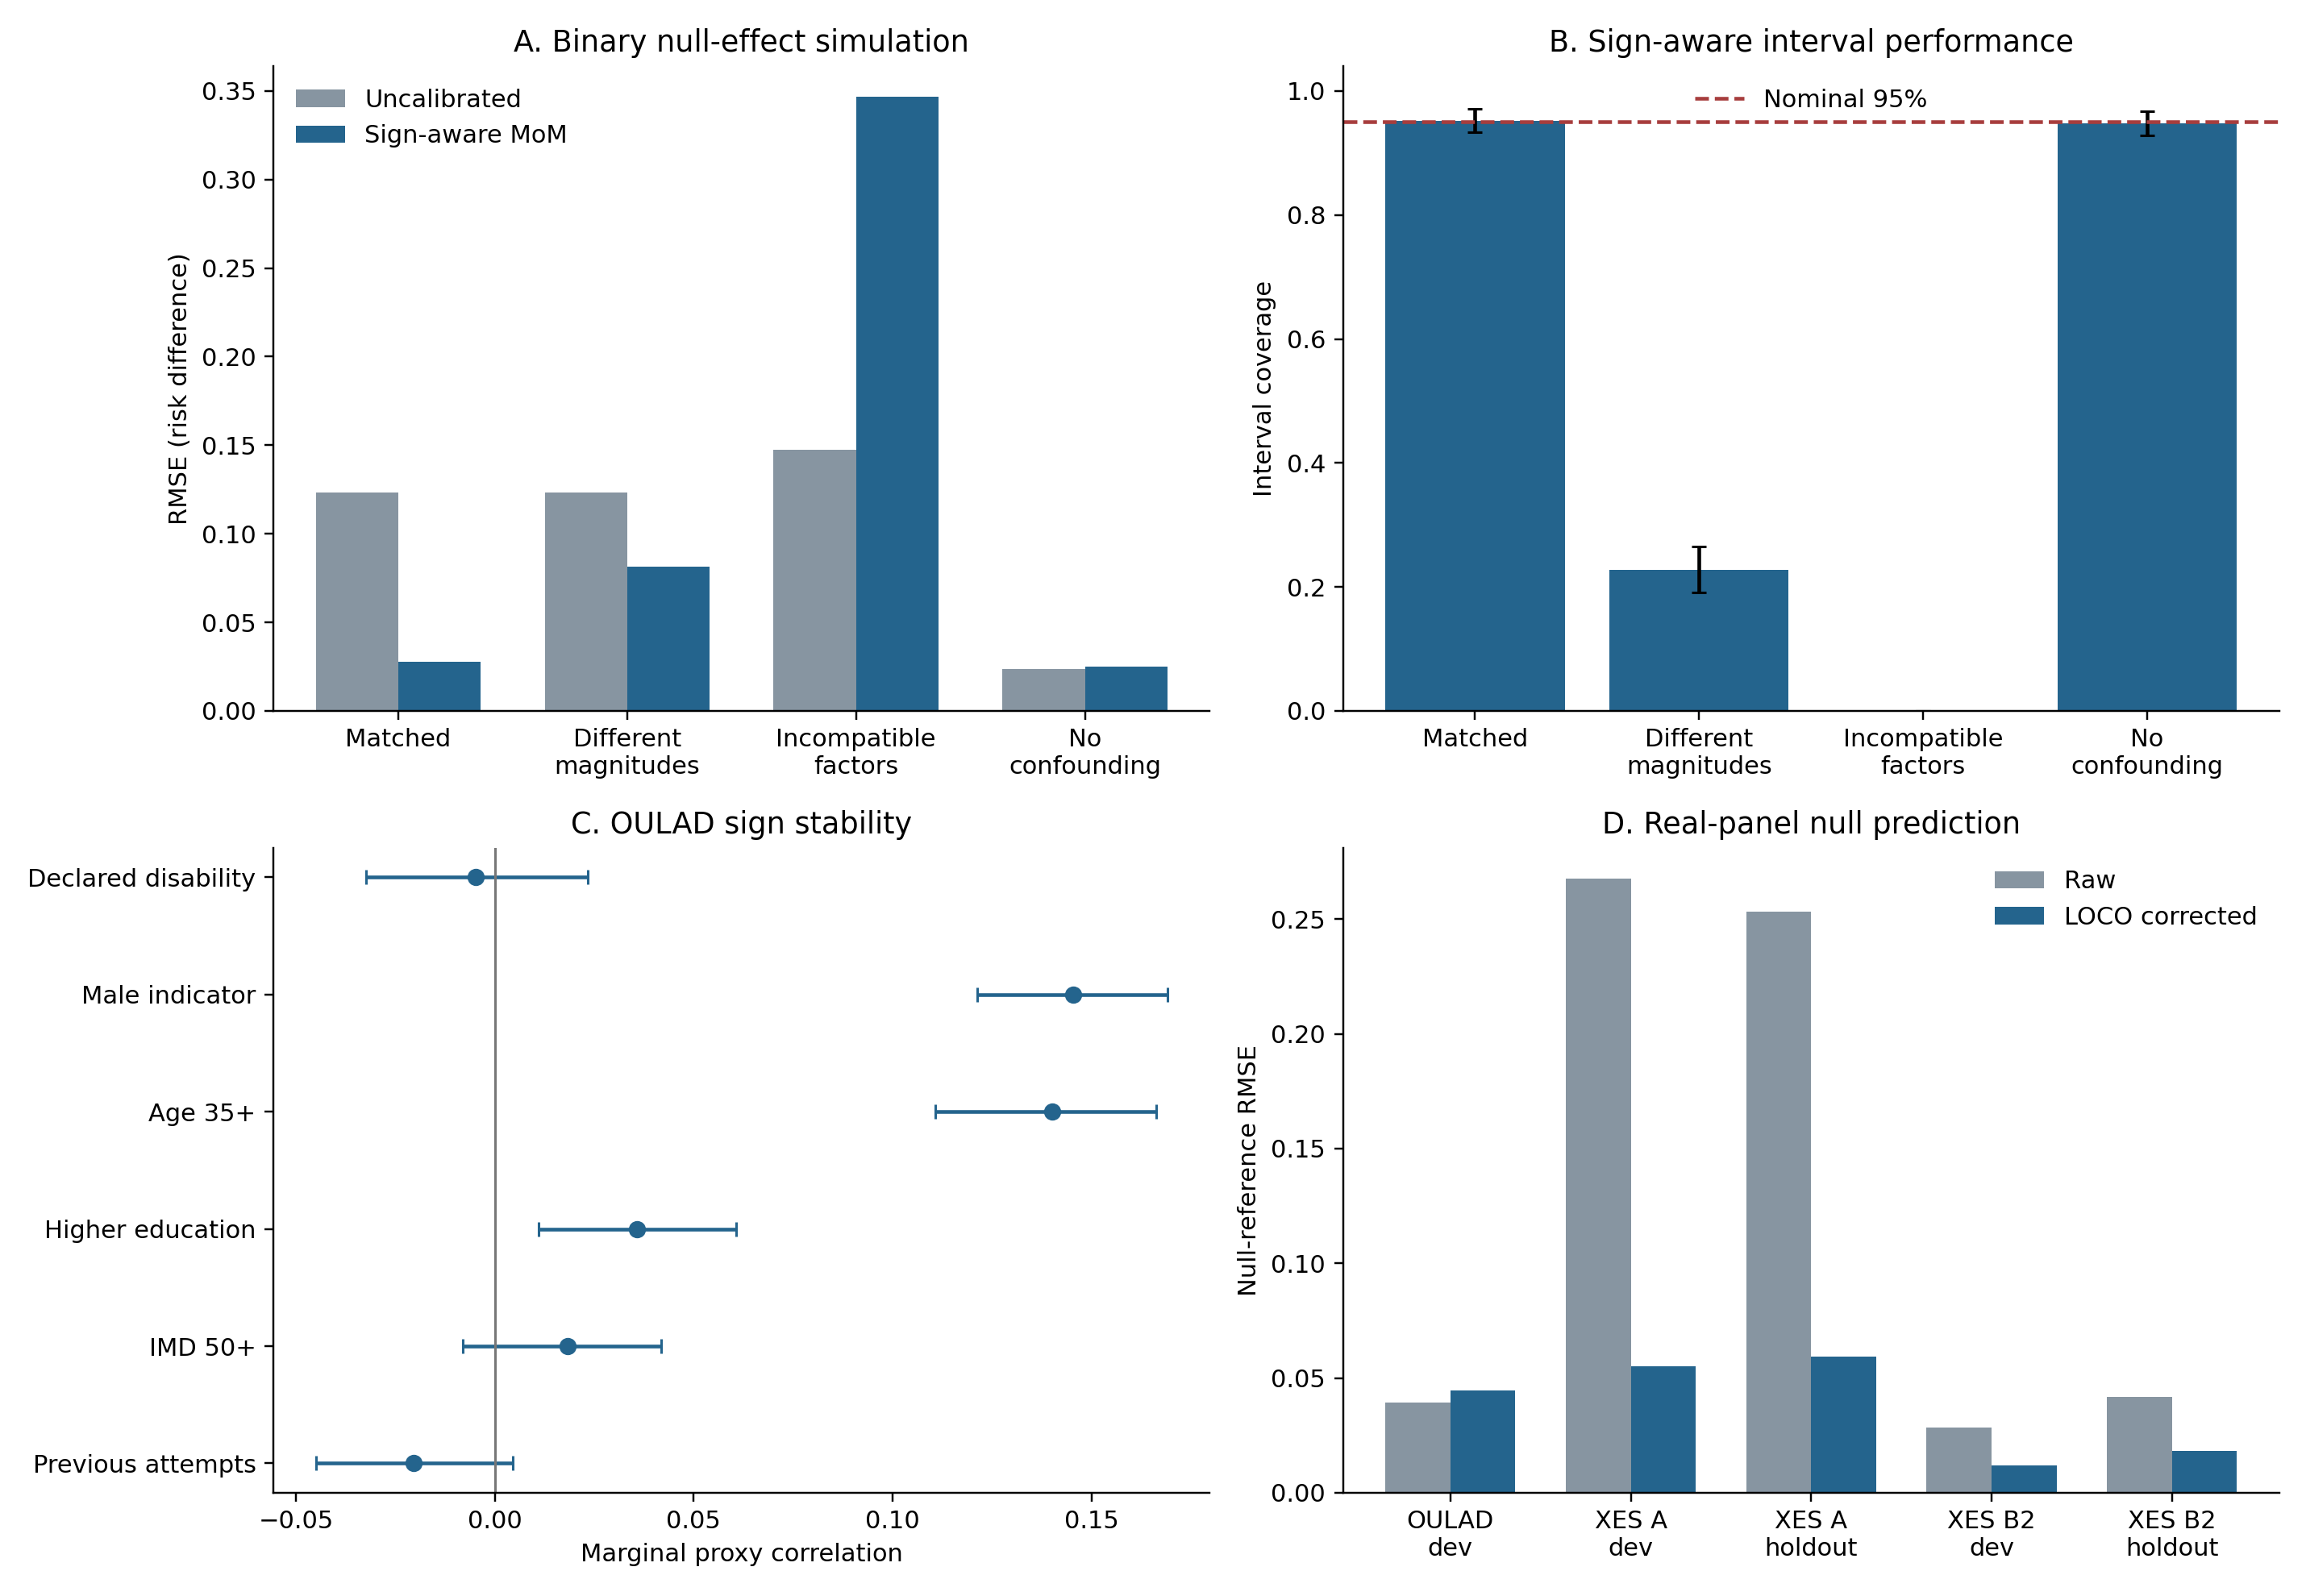
\includegraphics[width=\textwidth]{audit_summary.png}
\caption{Conditional simulation performance and real-panel diagnostics. Top: binary known-truth RMSE and nominal coverage (coverage bars show $\pm1.96$ Monte Carlo SE). Bottom left: OULAD cluster-bootstrap marginal correlations on full training keys. Bottom right: null-reference error before and after leave-one-control-out correction. Real-panel checks do not identify target bias.}\label{fig:audit-summary}\end{figure}